\section{Exploratory Budget Extension}
After inspecting the primary replay results, we specified a separate budget extension to test whether the short-budget comparison persists when more reference measurements are affordable. The extension protocol was recorded before its own execution, but after the primary analysis; it is therefore exploratory. It does not replace the original grid. It fixes the unweighted tilt-0.50 replay, validation cost 5, all previous-year calibration, budgets 48, 144, 480 and 1,440, and 500 repetitions with a new seed. The same unit-channel packet bank is reused across the four budgets and all five policies. All outcomes from this grid are reported, including those unfavourable to two-channel KG.

\begin{table}[htbp]
\centering\small\begin{tabular}{lrrrrr}
\toprule
Budget & Ord. KG & Two KG & Balanced & Val. only & Uniform \\
\midrule
48 & 0.1794 & 0.1957 & 0.1972 & 0.1986 & 0.1988 \\
144 & 0.1593 & 0.1867 & 0.1897 & 0.1882 & 0.1815 \\
480 & 0.1367 & 0.1500 & 0.1800 & 0.1635 & 0.1605 \\
1440 & 0.1242 & 0.0907 & 0.1499 & 0.1229 & 0.1380 \\
\bottomrule
\end{tabular}

\caption{Exploratory budget extension: mean severity regret, 500 paired repetitions at each budget. This is a separate run from the 1,000-repetition primary grid. The complete CSV includes actual spending and paired Monte Carlo intervals.}
\end{table}

Two-channel KG remains worse than ordinary KG at budgets 48, 144 and 480. At budget 1,440, the comparison reverses: regret is 0.09070 versus 0.12422, a paired difference of $-0.03352$ with 95\% Monte Carlo interval [$-0.03793$,$-0.02910$]. This is evidence of a budget-dependent comparison within the specified replay, not a measured NHS cost threshold. At budgets 480 and 1,440, two-channel KG spends all additional resources on validation. The improvement must not be described as successful balancing of two channels. At 1,440, uniform validation also uses only validation, spends the same budget, and has regret 0.12288; the comparison with KG concerns which units receive those reference packets. The budget is 30 ordinary-packet cost equivalents per area, or 288 validation packets in total at cost 5, on top of the shared initial observations. A real price per completed packet is not inferred.

\begin{figure}[htbp]
\centering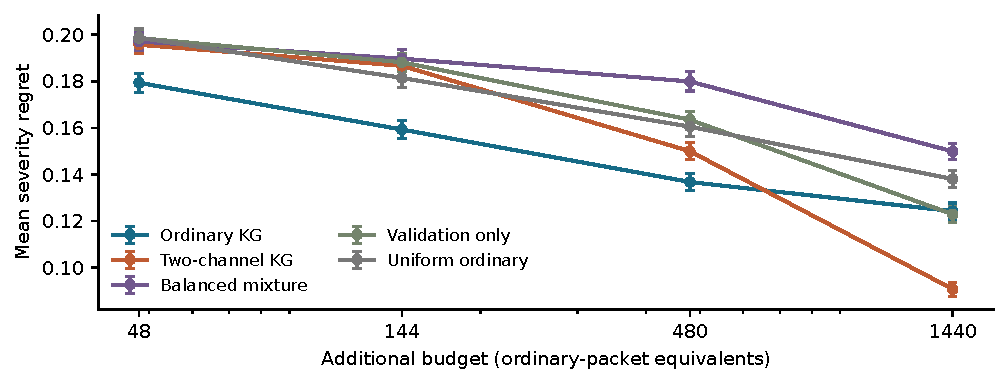
\includegraphics[width=\textwidth]{figures/budget_extension.pdf}
\caption{Exploratory budget sensitivity on one controlled replay mechanism. Error bars are 95\% Monte Carlo intervals. All four budgets were specified before running this extension. Ordinary-only policies cannot access validation; the balanced mixture and validation-only policy provide comparisons with that access.}
\end{figure}

\section{Estimation, Cost and Misspecification Diagnostics}
The MSE/regret comparison makes the target dependence of acquisition tangible. MSE averages squared level errors across every unit; severity regret evaluates only the selected set relative to the oracle with the same quota. A small reduction in aggregate MSE can coexist with a less accurate ordering around the selection boundary. The replay comparisons below are descriptive effects of full policies. They do not isolate how much of the difference is due to Gaussian approximation, prior calibration, per-packet noise, cost or myopic action choice.

\begin{table}[htbp]
\centering\small\begin{tabular}{lrrrrr}
\toprule
Scenario & Ord. loss & Two loss & Ord. MSE & Two MSE & Val. cost \\
\midrule
Uniform & 0.1124 & 0.1124 & 0.01802 & 0.01802 & 0.0\% \\
Tilt 0.25 & 0.1570 & 0.1755 & 0.02116 & 0.02092 & 90.2\% \\
Tilt 0.50 & 0.1615 & 0.1857 & 0.02183 & 0.02129 & 97.2\% \\
Weighted tilt & 0.1773 & 0.1959 & 0.02250 & 0.02194 & 97.2\% \\
Biased validation & 0.1612 & 0.2226 & 0.02182 & 0.02308 & 97.2\% \\
\bottomrule
\end{tabular}

\caption{Primary replay at budget 144 and validation cost 5. ``Ord.'' and ``Two'' refer to ordinary-only and two-channel KG with matched bias-aware inference. Validation cost is the fraction of the two-channel policy's budget spent on that channel. Target MSE and selection loss are distinct.}
\end{table}

\begin{figure}[htbp]
\centering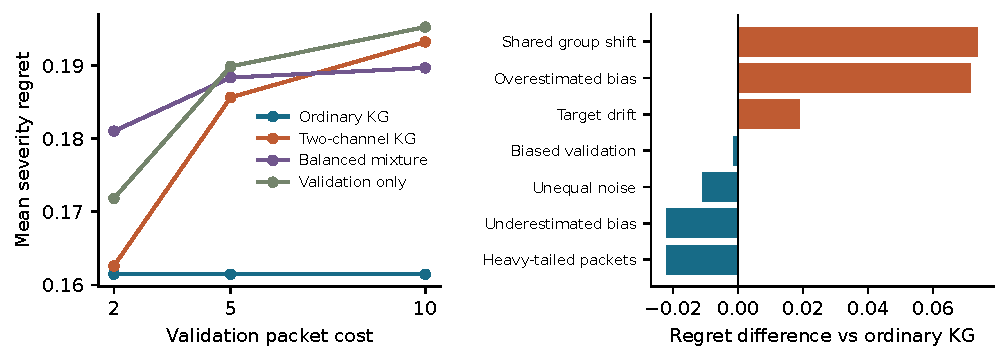
\includegraphics[width=\textwidth]{figures/cost_and_stress.pdf}
\caption{Left: validation-cost sensitivity on tilt-0.50 replay at budget 144. Right: synthetic stress-world regret differences at budget 120 and cost 5; positive values favour ordinary KG. All stress results remain in the numerical release, including small or adverse comparisons.}
\end{figure}

\section{Research Transparency}
This study uses public aggregate NHS data and public-use BRFSS records. It conducts no new recruitment, intervention or private-data linkage. The computational benchmark does not attribute individuals' mental health to their jobs and does not diagnose a clinical condition. Source: CDC BRFSS. This independent research and its conclusions are not endorsed by CDC, HHS, the United States Government or NHS organisations. Existing source terms continue to govern original materials; a licence for newly authored code does not relicense agency materials.

AI assistance was used extensively for literature discovery, mathematical derivation, code generation, numerical auditing, analysis and manuscript preparation. Automated checks and independent implementations are documented; they do not replace the named author's responsibility for reviewing the manuscript, verifying references, understanding the analysis and approving any submission. No external stakeholder co-design, ethics approval, funding award or deployment is claimed. No real institutional allocation has been made from the research. Authorship and any necessary institutional declarations must accurately reflect the actual work and affiliation when submitted.

The source package contains runnable experiment scripts, derived public-data frames, complete summary CSVs, a results workbook, acquisition/source manifests, numerical-verification scripts, local analysis protocols and source snapshots for the primary runs. Detailed simulation metrics can be regenerated with the stored seeds. The separate exploratory extension also retains replication-level arrays. Working-directory paths and personal identifiers are excluded from the anonymous PDF text. Public-data access, re-download and source validation depend on continued availability of the cited official releases; included derived-data reproduction does not require private credentials or a GPU.
